% =====================================================================
%  Legendre's Conjecture in Function Fields:
%  the Classical Range, Full Monodromy, and the Open Range q <= d-2
%  Version v7 (revises v6, DOI 10.5281/zenodo.23179113, and v5, DOI 10.5281/zenodo.18705744)
% =====================================================================
\documentclass[11pt,a4paper]{article}

\usepackage[top=28mm,bottom=28mm,left=25mm,right=25mm]{geometry}
\usepackage[T1]{fontenc}
\usepackage{lmodern}
\usepackage{amsmath,amssymb,amsthm,mathtools}
\usepackage{graphicx}
\usepackage{booktabs}
\usepackage[dvipsnames]{xcolor}
\usepackage{enumitem}
\usepackage[colorlinks=true,linkcolor=MidnightBlue,citecolor=MidnightBlue,urlcolor=MidnightBlue]{hyperref}

\newtheorem{theorem}{Theorem}[section]
\newtheorem{lemma}[theorem]{Lemma}
\newtheorem{proposition}[theorem]{Proposition}
\newtheorem{corollary}[theorem]{Corollary}
\newtheorem{conjecture}[theorem]{Conjecture}
\newtheorem*{theoremA}{Theorem 1}
\newtheorem*{theoremB}{Theorem 2}
\newtheorem*{theoremC}{Theorem 3}
\newtheorem*{conjectureA}{Conjecture}
\theoremstyle{definition}
\newtheorem{definition}[theorem]{Definition}
\theoremstyle{remark}
\newtheorem{remark}[theorem]{Remark}

\newcommand{\Fq}{\mathbb{F}_q}
\newcommand{\Fqbar}{\overline{\mathbb{F}}_q}
\newcommand{\A}{\mathbb{A}}
\newcommand{\Gal}{\mathrm{Gal}}
\newcommand{\Tr}{\mathrm{Tr}}
\newcommand{\disc}{\mathrm{disc}}
\newcommand{\Ggeom}{G_{\mathrm{geom}}}
\newcommand{\Nirr}{N_{\mathrm{irr}}}
\newcommand{\cI}{\mathcal{I}}
\newcommand{\cM}{\mathcal{M}}
\newcommand{\cH}{\mathcal{H}}
\newcommand{\ba}{\mathbf{a}}

% numbers generated from the data by code/make_tables.py
\newcommand{\VerTwo}{20}
\newcommand{\VerThree}{10}
\newcommand{\VerFour}{10}
\newcommand{\VerFive}{8}
\newcommand{\AllQd}{8}
\newcommand{\AllQdNext}{9}
\newcommand{\MinRatioOpen}{0.375}
\newcommand{\MinRatioCase}{(2,6)}
\newcommand{\MaxDeficit}{0.51}
\newcommand{\MaxDeficitCase}{(2,5)}


\title{\textbf{Legendre's Conjecture in Function Fields:\\
the Classical Range, Full Monodromy,\\ and the Open Range $q\le d-2$}\\[4pt]
\large Version v7 of \textit{The Geometry of Prime Vacuums}}
\author{Ruqing Chen\\[3pt]
\small GUT Geoservice Inc., Montr\'eal, Canada\\
\small \texttt{ruqing@hotmail.com}}
\date{October 2026\\[2pt]\small Code and data: \url{https://github.com/Ruqing1963/legendre-function-field}}

\begin{document}
\maketitle

\begin{abstract}
For a monic polynomial $f\in\Fq[t]$ of degree $d$, the \emph{Legendre interval}
$\cI_f=\{f^2+s:\ \deg s\le d\}$ is the function field analogue of $[n^2,(n+1)^2]$.
We record the explicit form of a classical estimate (Hayes characters and Weil's theorem):
$|\sum_{P\in\cI_f}\Lambda(P)-q^{d+1}|\le(d-2)(q^d-q)$ in every characteristic.
Together with a bound for prime powers in $\cI_f$, it shows that $\cI_f$ contains an
irreducible polynomial whenever $q\ge d-1$. This supersedes all thresholds of earlier versions
of this preprint, which overlooked it. The genuine analogue of Legendre's conjecture, with $q$
fixed and $d\to\infty$, lies in the remaining range $q\le d-2$.
We examine every Legendre interval for $q=2$ with $d\le\VerTwo$, for $q=3$ with $d\le\VerThree$,
for $q=4$ with $d\le\VerFour$, and for $q=5$ with $d\le\VerFive$. All of them contain
irreducible polynomials, so the analogue of Legendre's conjecture holds for every $q$ when
$d\le\AllQd$. Over odd $q$ the variance of the prime count across intervals is already close
to the Keating--Rudnick prediction $(d-2)q^{d+1}$, proved only for $q\to\infty$, and the
smallest normalized count approaches $1$ as $d$ grows. We state a conjecture with a heuristic
based on these observations. We also give a self-contained proof that the geometric monodromy
group of the family is $S_{2d}$ for $p>2d$, an exact twisted-variety identity, closed formulas
for $d\le3$, and a list of corrections to v5 and v6.
\end{abstract}

\tableofcontents
\bigskip

% =====================================================================
\section{Introduction}\label{sec:intro}
% =====================================================================

\subsection{The question}
Legendre's conjecture asserts that there is a prime between $n^2$ and $(n+1)^2$ for every
$n\ge1$. It is open. The best unconditional result on prime gaps gives primes in
$[x,x+x^{0.525}]$ \cite{BHP2001}, and even the Riemann hypothesis only gives intervals of
length about $\sqrt x\log x$.

In $\Fq[t]$ put $|g|=q^{\deg g}$. For monic $f$ of degree $d$, the polynomials $g$ with
$|g-f^2|\le|f|$ form the \emph{Legendre interval}
\[
  \cI_f=\{\,f^2+s:\ s\in\Fq[t],\ \deg s\le d\,\},\qquad |\cI_f|=q^{d+1}.
\]
Its elements are the monic polynomials of degree $2d$ whose coefficients of
$t^{2d-1},\dots,t^{d+1}$ agree with those of $f^2$. We write
\[
  \Nirr(f)=\#\{P\in\cI_f:\ P\text{ irreducible}\},\qquad
  \Psi(f)=\sum_{P\in\cI_f}\Lambda(P),
\]
where $\Lambda(P)=\deg\pi$ if $P=\pi^r$ with $\pi$ irreducible and $\Lambda(P)=0$ otherwise.
Then $2d\,\Nirr(f)=\Psi(f)-E(f)$, where $E(f)$ collects the prime powers $\pi^r$, $r\ge2$.
The prime polynomial theorem predicts $\Nirr(f)\approx q^{d+1}/(2d)$.
\emph{Does every Legendre interval contain an irreducible polynomial?}

\subsection{What is known, and what this paper adds}

\paragraph{The classical range $q\ge d-1$.}
The interval $\cI_f$ is a class of polynomials with $\ell=d-1$ prescribed leading coefficients.
Such classes are the fibres of Hayes's characters \cite{Hayes1965}, whose $L$-functions are
polynomials of degree at most $\ell-1$ satisfying the Riemann hypothesis by Weil's theorem.
This gives explicit bounds for irreducible polynomials with prescribed leading coefficients
(Hsu \cite{Hsu1996}, Cohen \cite[Thm.~2.1]{Cohen2005}; see \cite[Cors.~1--2]{Gao2021}).
For Legendre intervals they read as follows.

\begin{theoremA}[Section~\ref{sec:classical}]
For every prime power $q$ and every monic $f$ of degree $d\ge2$,
\[
  \bigl|\Psi(f)-q^{d+1}\bigr|\le(d-2)\,(q^d-q).
\]
Consequently $\Nirr(f)\ge1$ whenever $q\ge d-1$, in every characteristic.
\end{theoremA}

The first statement is classical in substance; we give a short proof to fix constants.
The consequence for $q\in\{d-1,d\}$ uses an elementary bound on $E(f)$ (Lemma~\ref{lem:E}).
At $q=d-2$ the estimate gives nothing, because the main term $q^{d+1}$ and the error
$(d-2)q^d$ are then equal. This is the function field form of the familiar fact that the
Riemann hypothesis \emph{just} fails to reach Legendre's conjecture over $\mathbb Z$.

Earlier versions of this preprint missed Theorem~1. Version v5 claimed the threshold
$q>(8d)^{2d+6}$ without valid proof, and version v6 proved thresholds such as
$q>1.65\times10^4$ for $d=4$. Both are far weaker than $q\ge d-1$; see Appendix~\ref{app:errata6}.
The asymptotic $\Nirr=q^{d+1}/2d+O_d(q^{d+1/2})$ for fixed $d$, the ``main theorem'' of v5, is
contained in Theorem~1 and also in the short-interval theorem of Bank, Bary-Soroker and
Rosenzweig \cite{BBR2015}. Their result, and Sawin's sharper bound \cite{Sawin2021}, concern
shorter intervals or larger $q$; at the Legendre length the classical estimate is the relevant one.

\paragraph{The open range $q\le d-2$.}
Here no general method is known. Reversing polynomials turns $\cI_f$ into a residue class modulo
$t^{d}$ among polynomials of degree $2d$, at level of distribution exactly $1/2$. Sawin and
Shusterman \cite{SawinShusterman2022} pass level $1/2$ for squarefree moduli when $q$ is large
compared with $p$, but the moduli $t^d$ are not covered. Results on prescribed coefficients
\cite{Pollack2013,Ha2016} allow far fewer than the $d-1$ coefficients needed here.
We therefore study this range by exhaustive computation.

\begin{theoremB}[Section~\ref{sec:open}]
Every Legendre interval over $\Fq$ contains an irreducible polynomial when
$q=2,\ d\le\VerTwo$; $q=3,\ d\le\VerThree$; $q=4,\ d\le\VerFour$; $q=5,\ d\le\VerFive$.
Together with Theorem~1, the function field analogue of Legendre's conjecture holds for
every prime power $q$ when $d\le\AllQd$.
\end{theoremB}

The computations also measure how the prime count fluctuates from interval to interval.
For odd $q$ the Legendre intervals are \emph{all} the intervals of length $q^{d+1}$ in degree
$2d$, and Keating and Rudnick \cite{KR2014} proved that the variance of $\Psi$ over them is
$\sim(d-2)q^{d+1}$ as $q\to\infty$. We find this already accurate for $q=3$ and $q=5$
(Table~\ref{tab:open}). A Gaussian model with this variance predicts that the smallest
normalized count tends to $1$ as $d\to\infty$, which is what the data show (Figure~\ref{fig:minratio}).
This leads to:

\begin{conjectureA}[Section~\ref{sec:conjecture}]
For every prime power $q$ and every $d\ge1$, every Legendre interval in $\Fq[t]$ contains an
irreducible polynomial. Moreover, for fixed $q$,
$\min_{f}\Psi(f)/q^{d+1}\to1$ as $d\to\infty$.
\end{conjectureA}

\paragraph{Other results kept from v6.}
For $p>2d$ we give a self-contained proof that the geometric monodromy group of
$f^2+\sum_{i\le d}a_it^i$ is $S_{2d}$, for every monic $f$ (Theorem~\ref{thm:monodromy}).
We also prove an exact identity $\Psi(f)=\#W(\Fq)$ for an explicit twisted root variety $W$
(Theorem~\ref{thm:identity}), and closed formulas for $\Nirr$ when $d\le3$
(Section~\ref{sec:small}). These are not needed for Theorems~1 and~2, but they explain the
factorization statistics in Figure~\ref{fig:cheb} and give independent checks of the code.

\subsection{About this revision}
Appendix~\ref{app:errata} lists the errors of v5, and Appendix~\ref{app:errata6} the
omissions of v6 corrected here. The main changes from v6 are Theorem~1, which replaces all
of v6's explicit thresholds, and the new computations of Section~\ref{sec:open}.

% =====================================================================
\section{The classical range}\label{sec:classical}
% =====================================================================

\subsection{Hayes classes}
For monic $g$ of degree $k$ put $\tilde g(u)=u^kg(1/u)\in\Fq[u]$; its constant term is $1$.
Let $\ell\ge0$ and let $\mathcal G_\ell$ be the group of power series $1+c_1u+\dots$ modulo
$u^{\ell+1}$, of order $q^\ell$. The map $g\mapsto[g]:=\tilde g\bmod u^{\ell+1}$ is
multiplicative, and $[g]$ records exactly the $\ell$ coefficients of $g$ below the leading one.
With $\ell=d-1$, $\cI_f$ is the set of monic $P$ of degree $2d$ with $[P]=[f^2]$.

\begin{lemma}\label{lem:hayes}
Let $\chi\ne1$ be a character of $\mathcal G_\ell$ and $\chi(g)=\chi([g])$ for monic $g$.
Then $L(z,\chi)=\sum_{g\text{ monic}}\chi(g)z^{\deg g}$ is a polynomial of degree at most $\ell-1$,
and its inverse roots have absolute value $q^{1/2}$ or $1$.
\end{lemma}

\begin{proof}
For $k\ge\ell$ the map $g\mapsto[g]$ from monic polynomials of degree $k$ onto $\mathcal G_\ell$ has
all fibres of size $q^{k-\ell}$, so $\sum_{\deg g=k}\chi(g)=0$. Hence $L$ is a polynomial of degree
$\le\ell-1$. These are $L$-functions of characters of a ray class group of $\Fq(t)$, with conductor
supported at the place $t=\infty$, and the Riemann hypothesis for them is Weil's theorem; see
\cite{Hayes1965} and \cite[\S4]{KR2014}, where they appear as even Dirichlet characters modulo
$u^{\ell+1}$ after the substitution $t\mapsto1/u$.
\end{proof}

\begin{theorem}[Theorem 1, first part]\label{thm:classical}
For every $q$ and every monic $f$ of degree $d\ge2$, $|\Psi(f)-q^{d+1}|\le(d-2)(q^d-q)$.
For $d=2$ this means $\Psi(f)=q^3$ exactly.
\end{theorem}

\begin{proof}
Let $\ell=d-1$ and $n=2d$. By orthogonality,
$\Psi(f)=q^{-\ell}\sum_\chi\bar\chi([f^2])\sum_{\deg P=n}\Lambda(P)\chi(P)$.
The trivial character contributes $q^{-\ell}\cdot q^{n}=q^{d+1}$. For $\chi\ne1$ write
$L(z,\chi)=\prod_{i}(1-\omega_iz)$ with at most $\ell-1$ factors. Taking the logarithmic
derivative gives $\sum_{\deg P=n}\Lambda(P)\chi(P)=-\sum_i\omega_i^n$, of absolute value at most
$(\ell-1)q^{n/2}=(d-2)q^d$. There are $q^\ell-1$ nontrivial characters, each weighted by $q^{-\ell}$, so
$|\Psi(f)-q^{d+1}|\le(1-q^{-(d-1)})(d-2)q^d=(d-2)(q^d-q)$.
\end{proof}

\begin{lemma}[Prime powers in a Legendre interval]\label{lem:E}
Let $E(f)=\Psi(f)-2d\,\Nirr(f)$. Then
\[
 E(f)\le d\,q^{a}+2q^{\lfloor 2d/3\rfloor},\qquad a=\begin{cases}1,& p \text{ odd},\\ \lceil (d+1)/2\rceil, & p=2.\end{cases}
\]
Moreover $E(f)\le\sum_{e\mid2d,\,e<2d}q^e<q^d+2q^{\lfloor2d/3\rfloor}$ in all cases.
\end{lemma}

\begin{proof}
$E(f)$ is the sum of $\deg\pi$ over irreducible $\pi$ of degree $e=2d/r$, $r\ge2$, with
$\pi^r\in\cI_f$. Since $e\cdot\#\{\pi:\deg\pi=e\}\le q^e$, the terms with $r\ge3$ contribute at most
$\sum_{e\le 2d/3}q^e<2q^{\lfloor2d/3\rfloor}$, and all terms together at most $\sum_{e\mid 2d,e<2d}q^e$.
For $r=2$, write $\pi=t^d+\pi_{d-1}t^{d-1}+\dots+\pi_0$. If $p$ is odd, the coefficient of
$t^{2d-j}$ in $\pi^2$ is $2\pi_{d-j}+\Phi_j(\pi_{d-1},\dots,\pi_{d-j+1})$ for a universal
polynomial $\Phi_j$, so the $d-1$ prescribed coefficients determine $\pi_{d-1},\dots,\pi_1$, and at
most $q$ polynomials $\pi$ qualify. If $p=2$, then $\pi^2=\sum_i\pi_i^2t^{2i}$, the prescribed
coefficients determine $\pi_{d-1},\dots,\pi_{d-\lfloor(d-1)/2\rfloor}$, and at most
$q^{\lceil(d+1)/2\rceil}$ polynomials qualify. Each contributes $d$.
\end{proof}

\begin{corollary}[Theorem 1, second part]\label{cor:classical}
If $q\ge d-1$, then $\Nirr(f)\ge1$ for every monic $f$ of degree $d$.
\end{corollary}

\begin{proof}
For $d\le2$ see Theorem~\ref{thm:small}. Let $d\ge3$. By Theorem~\ref{thm:classical},
$2d\,\Nirr(f)\ge q^{d+1}-(d-2)(q^d-q)-E(f)=q^d(q-d+2)+(d-2)q-E(f)$.

If $q\ge d$ the right side is at least $2q^d+(d-2)q-E(f)$, which is positive because
$E(f)<q^d+2q^{\lfloor2d/3\rfloor}\le 2q^d$ (note $\lfloor 2d/3\rfloor\le d-1$ and $q\ge2$).

If $q=d-1$ the right side is $q^d+(d-2)q-E(f)$. For odd $q$ (so $d\ge4$),
Lemma~\ref{lem:E} gives $E(f)\le dq+2q^{d-2}$, since $\lfloor2d/3\rfloor\le d-2$ for $d\ge4$;
and $2q+2q^{d-2}<q^d$ because $q\ge3$. For even $q$ we have $d=q+1$ odd and
$E(f)\le d\,q^{(d+1)/2}+2q^{\lfloor2d/3\rfloor}$, which is less than $q^d$ for $d\ge5$, $q\ge4$.
The single remaining case $(q,d)=(2,3)$ is checked directly: $\Nirr=2$ for every $f$
(Table~\ref{tab:open}).
\end{proof}

\begin{remark}
The second part of Theorem~1 is sharp for this method: when $q=d-2$ the lower bound
$q^d(q-d+2)+(d-2)q-E(f)$ equals $q^2-E(f)$, which is negative. Theorem~1 also gives
$\Nirr=q^{d+1}/2d+O(dq^d)$ for fixed $d$, with an explicit constant. This is stronger than
the error $O_d(q^{d+1/2})$ of \cite{BBR2015}. Sawin's bound \cite{Sawin2021} has the better
$q$-exponent $q^{d/2+1}$ but a constant of size $(2d+2)^{3d}$; it is the right tool for $q$ very
large compared with $d$, not for existence.
\end{remark}

All $174$ exact counts with $q>d$ computed for v6 satisfy the bounds of Theorem~\ref{thm:classical}
(\texttt{data/interval\_counts.csv}).

% =====================================================================
\section{The open range $q\le d-2$}\label{sec:open}
% =====================================================================

\subsection{Method}
By Theorem~1 only the pairs with $q\le d-2$ need checking. The substitutions
$t\mapsto\lambda t+b$ ($\lambda\in\Fq^\times$, $b\in\Fq$) preserve irreducibility and map Legendre
intervals to Legendre intervals: $f$ goes to $\lambda^{-d}f(\lambda t+b)$. We list all distinct
Legendre intervals, group them into orbits under these substitutions, and for one representative
of each orbit we test every element for irreducibility. We also compute $E(f)$ by enumerating the
candidate prime powers, so $\Psi(f)=2d\,\Nirr(f)+E(f)$ is known exactly.

Field arithmetic uses addition and multiplication tables for $\Fq$, so prime and non-prime $q$
are handled by the same code. Irreducibility is decided by Ben-Or's test: a monic $P$ of degree $n$
is irreducible if and only if $\gcd(t^{q^i}-t,P)=1$ for $1\le i\le n/2$. The implementation is
cross-checked against an independent distinct-degree factorization for prime $q$, against a
pure-Python implementation for $q=4,8,9$, and against the twisted-variety count of
Section~\ref{sec:twisted}. A further check is exact: for odd $q$ every residue class of
leading coefficients is a Legendre interval, so the orbit-weighted sum of $\Psi$ must equal
$q^{d-1}\cdot q^{d+1}$. It does in every case tested.

In characteristic $2$ the Legendre intervals form a thin subfamily. Indeed $f^2=\sum c_i^2t^{2i}$,
so every prescribed coefficient in an odd position is $0$. There are only $q^{\lfloor(d-1)/2\rfloor}$
Legendre intervals, which is why $q=2$ can be pushed much further than $q=3$.

\subsection{Results}

\begin{table}[ht]
\centering\small
\begin{tabular}{rrrrrrrr}
\toprule
$q$ & $d$ & intervals & orbits & $\min N_{\rm irr}$ & ratio & $\mathrm{Var}\,\Psi/q^{d+1}$ & $d-2$ \\
\midrule
2 & 2 & 1 & 1 & 1 & 0.500 & 0.00 & -- \\
2 & 3 & 2 & 1 & 2 & 0.750 & 0.00 & -- \\
2 & 4 & 2 & 2 & 2 & 0.500 & 2.00 & 2 \\
2 & 5 & 4 & 2 & 5 & 0.781 & 1.25 & 3 \\
2 & 6 & 4 & 3 & 4 & 0.375 & 15.56 & 4 \\
2 & 7 & 8 & 4 & 13 & 0.711 & 7.72 & 5 \\
2 & 8 & 8 & 6 & 28 & 0.875 & 1.59 & 6 \\
2 & 9 & 16 & 8 & 47 & 0.826 & 5.77 & 7 \\
2 & 10 & 16 & 10 & 92 & 0.898 & 7.91 & 8 \\
2 & 11 & 32 & 16 & 167 & 0.897 & 15.35 & 9 \\
2 & 12 & 32 & 20 & 296 & 0.867 & 20.74 & 10 \\
2 & 13 & 64 & 32 & 593 & 0.941 & 11.47 & 11 \\
2 & 14 & 64 & 36 & 1102 & 0.942 & 17.37 & 12 \\
2 & 15 & 128 & 64 & 2106 & 0.964 & 11.86 & 13 \\
2 & 16 & 128 & 72 & 3952 & 0.965 & 15.22 & 14 \\
2 & 17 & 256 & 128 & 7580 & 0.983 & 13.88 & 15 \\
2 & 18 & 256 & 136 & 14310 & 0.983 & 19.71 & 16 \\
2 & 19 & 512 & 256 & 27290 & 0.989 & 17.65 & 17 \\
2 & 20 & 512 & 272 & 51841 & 0.989 & 19.45 & 18 \\
\addlinespace
3 & 5 & 81 & 18 & 63 & 0.864 & 1.80 & 3 \\
3 & 6 & 243 & 48 & 156 & 0.856 & 4.85 & 4 \\
3 & 7 & 729 & 135 & 440 & 0.939 & 4.44 & 5 \\
3 & 8 & 2187 & 378 & 1165 & 0.947 & 5.50 & 6 \\
3 & 9 & 6561 & 1143 & 3123 & 0.952 & 6.66 & 7 \\
3 & 10 & 19683 & 3321 & 8600 & 0.971 & 7.89 & 8 \\
3 & 11$^\dagger$ & 59049 & 30 & 23996 & 0.993 & -- & 9 \\
\addlinespace
4 & 6 & 16 & 3 & 1280 & 0.938 & 9.01 & 4 \\
4 & 7 & 64 & 8 & 4530 & 0.968 & 9.36 & 5 \\
4 & 8 & 64 & 12 & 15936 & 0.973 & 13.25 & 6 \\
4 & 9 & 256 & 24 & 57886 & 0.994 & 6.36 & 7 \\
4 & 10 & 256 & 28 & 208536 & 0.994 & 10.47 & 8 \\
\addlinespace
5 & 7 & 15625 & 815 & 27579 & 0.988 & 4.45 & 5 \\
5 & 8 & 78125 & 3940 & 121334 & 0.994 & 5.51 & 6 \\
\bottomrule
\end{tabular}
\caption{The open range. ``Intervals'' is the number of distinct Legendre intervals and
``orbits'' the number examined after the affine reduction; rows marked $^\dagger$ examine a random
sample of orbits. The ratio is $\min_f 2d\,\Nirr(f)/q^{d+1}$. The variance column is the mean
of $(\Psi(f)-q^{d+1})^2/q^{d+1}$ over all Legendre intervals. For odd $q$ it is to be compared with
the Keating--Rudnick limit $d-2$ \cite{KR2014}, valid for $d\ge4$; for $q=2,4$ the Legendre intervals
are a special subfamily and no prediction applies. Rows with $q\ge d-1$ other than $q=2$ are omitted,
since Theorem~1 covers them. Source: \texttt{data/open\_regime\_summary.csv}.}
\label{tab:open}
\end{table}

\begin{theorem}[Theorem 2]\label{thm:computed}
Every Legendre interval over $\Fq$ contains an irreducible polynomial for $q=2$ and $d\le\VerTwo$,
$q=3$ and $d\le\VerThree$, $q=4$ and $d\le\VerFour$, and $q=5$ and $d\le\VerFive$. Consequently, for
every prime power $q$ and every $d\le\AllQd$, every Legendre interval contains an irreducible polynomial.
\end{theorem}

\begin{proof}
The first statement is the computation summarized in Table~\ref{tab:open}. For the second, let
$d\le\AllQd$. If $q\ge d-1$ apply Theorem~1. Otherwise $q\le d-2\le\AllQd-2$, so $q$ is one of the
prime powers listed, and the first statement applies.
\end{proof}

\begin{figure}[ht]
\centering
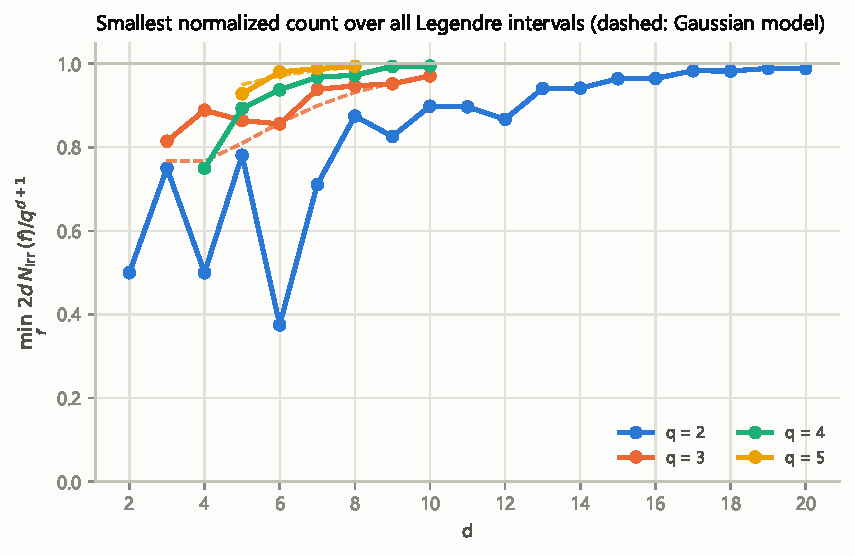
\includegraphics[width=0.85\linewidth]{../figures/fig5_open_min_ratio.pdf}
\caption{The smallest normalized count $\min_f2d\,\Nirr(f)/q^{d+1}$ in the open range.
It never reaches $0$ and approaches $1$ as $d$ grows.}
\label{fig:minratio}
\end{figure}

\begin{figure}[ht]
\centering
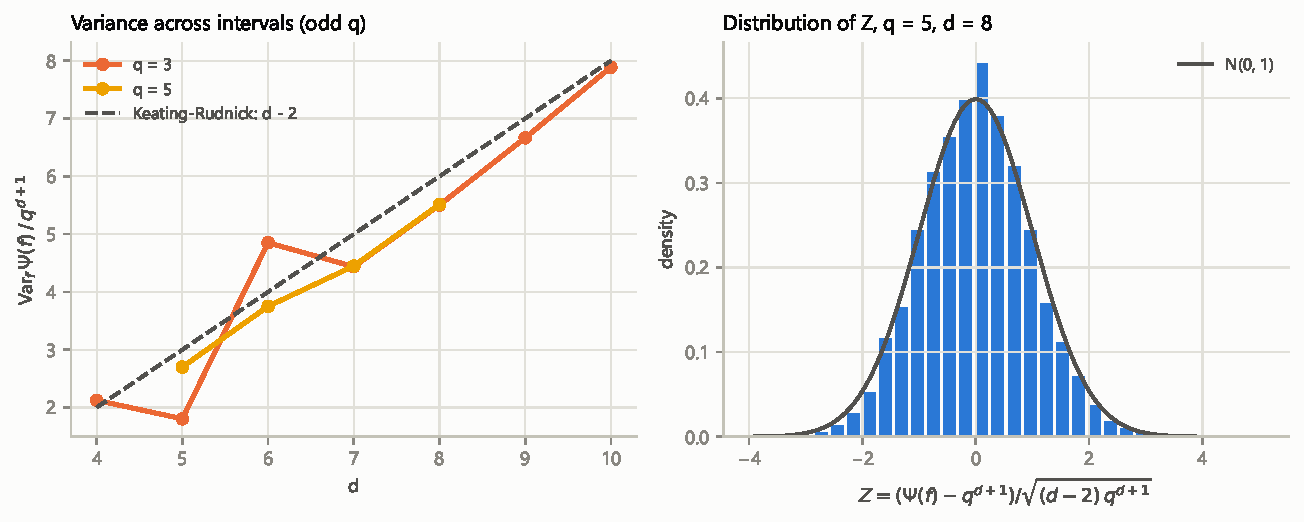
\includegraphics[width=\linewidth]{../figures/fig6_variance_kr.pdf}
\caption{Left: $\mathrm{Var}_f\Psi(f)/q^{d+1}$ over all Legendre intervals for odd $q$,
against the Keating--Rudnick limit $d-2$. Right: the distribution of
$Z=(\Psi(f)-q^{d+1})/\sqrt{(d-2)q^{d+1}}$ for the largest odd case, against the standard normal density.}
\label{fig:variance}
\end{figure}

\subsection{Observations}
\begin{enumerate}[label=(\roman*),nosep]
\item No empty Legendre interval occurs. The smallest normalized count in the open range is
      \MinRatioOpen, at $(q,d)=\MinRatioCase$.
\item For odd $q$ the empirical variance of $\Psi$ approaches $(d-2)q^{d+1}$, although Keating and
      Rudnick prove the asymptotic only for $q\to\infty$. For $q=3$ the relative deviation falls from
      $21\%$ at $d=6$ to $1.4\%$ at $d=10$; for $q=5$ it is at most $11\%$ for $5\le d\le8$.
\item In characteristic $2$ the Legendre intervals are a special subfamily and the variance
      fluctuates more. Small cases also show a downward bias in $\Nirr$, for example
      $\min_f 2d\,\Nirr/q^{d+1}=0.375$ at $(q,d)=(2,6)$. The bias fades as $d$ grows.
\end{enumerate}

% =====================================================================
\section{A conjecture}\label{sec:conjecture}
% =====================================================================

\begin{conjecture}\label{conj:main}
For every prime power $q$ and every $d\ge1$, every Legendre interval in $\Fq[t]$ contains an
irreducible polynomial. Moreover $\min_f\Psi(f)/q^{d+1}\to1$ as $d\to\infty$ with $q$ fixed.
\end{conjecture}

\paragraph{Heuristic.}
Model the values $\Psi(f)$ over the $q^{d-1}$ Legendre intervals ($q$ odd) as Gaussian with mean
$q^{d+1}$ and variance $(d-2)q^{d+1}$, as suggested by \cite{KR2014} and by Table~\ref{tab:open}.
The minimum of $N$ such variables is about $-\sqrt{2\log N}$ standard deviations, so
\[
 \min_f\frac{\Psi(f)}{q^{d+1}}\approx1-\sqrt{\frac{2(d-1)(d-2)\log q}{q^{d+1}}}\;\longrightarrow\;1 .
\]
The deficit is at most $\MaxDeficit$ over all $q\ge2$ and $d\ge3$, attained at $(q,d)=\MaxDeficitCase$,
so the model predicts no empty interval at all. Since $E(f)$ is at most of order $q^{\lfloor2d/3\rfloor}$ for odd $q$, the same
holds for $\Nirr$. The observed minima are consistent with the prediction (Figure~\ref{fig:minratio}).
The heuristic is not a proof. The Gaussian model is only known in the limit $q\to\infty$, and the
extreme tail of the distribution is exactly what a proof would have to control.

% =====================================================================
\section{The monodromy group}\label{sec:monodromy}
% =====================================================================

This section and the next two are kept from v6, with minor changes. Write
$\cM=\A^{d+1}$ with coordinates $\ba=(a_0,\dots,a_d)$ and $F(t,\ba)=f(t)^2+\sum_{i\le d}a_it^i$.

\subsection{Preliminaries}

\begin{lemma}[Membership in $\cI_f$]\label{lem:membership}
A monic $P\in\Fq[t]$ of degree $2d$ lies in $\cI_f$ if and only if its
coefficients of $t^{2d-1},\dots,t^{d+1}$ agree with those of $f^2$.
If $p>d-1$, this holds if and only if the power sums
$p_j(P)=\sum_{P(\rho)=0}\rho^j$ satisfy $p_j(P)=2\,p_j(f)$ for $1\le j\le d-1$.
\end{lemma}

\begin{proof}
Newton's identities express the power sums $p_1,\dots,p_{d-1}$ through the top $d-1$
coefficients, and conversely when $1,\dots,d-1$ are invertible. Finally $p_j(f^2)=2p_j(f)$.
\end{proof}

\begin{lemma}[Inertia at a simple node]\label{lem:node}
Let $R$ be a complete discrete valuation ring with algebraically closed residue
field of characteristic $\ne2$, fraction field $K$ and valuation $v$.
Let $P\in R[t]$ be monic of degree $n$ whose reduction $\bar P$ has exactly
one double root $\beta$ and $n-2$ simple roots, and suppose $v(\disc P)=1$.
Then the splitting field of $P$ over $K$ is a quadratic extension whose
Galois group acts on the roots of $P$ as a transposition.
\end{lemma}

\begin{proof}
Write $\bar P=(t-\beta)^2\bar L$ with $\bar L(\beta)\neq0$ and $\bar L$ squarefree.
By Hensel's lemma $P=QL$ with $Q,L\in R[t]$ monic lifting $(t-\beta)^2$ and $\bar L$,
and $L$ splits into linear factors over $R$.
Since $\disc P=\disc Q\cdot\disc L\cdot\mathrm{Res}(Q,L)^2$ and both
$\disc L$ and $\mathrm{Res}(Q,L)$ are units, $v(\disc Q)=1$.
An element of odd valuation is not a square in $K$, so $Q$ is irreducible over
$K$, and the nontrivial automorphism of its splitting field swaps the two roots of $Q$
and fixes the roots of $L$.
\end{proof}

\begin{lemma}[Primitivity and decomposition; cf.\ \cite{Turnwald1995,Muller1995}]\label{lem:luroth}
Let $K$ be a field, $G\in K[t]$ of degree $n\ge2$ with $G'\neq0$, and $x$
transcendental over $K$. If $\Gal(G(t)-x\,/\,K(x))$, acting on the roots of $G(t)-x$,
is imprimitive, then $G=g\circ h$ with $g,h\in K[t]$ and $\deg g,\deg h\ge2$.
\end{lemma}

\begin{proof}
Let $\tau$ be a root. Blocks containing $\tau$ correspond to fields $K(x)\subseteq L\subseteq K(\tau)$,
so imprimitivity gives a proper intermediate field $L$, and $L=K(h)$ by L\"uroth's theorem.
Since $x=G(\tau)$ is a polynomial in $\tau$, the place $\tau=\infty$ is the only
place of $K(\tau)$ above $x=\infty$, and it is $K$-rational; so is its restriction to $L$.
After a M\"obius transformation over $K$ we may take that place to be $h=\infty$.
Then $h$ has its only pole at $\tau=\infty$, so $h\in K[\tau]$, and likewise $x=g(h)$ with
$g\in K[X]$. Both degrees are $\ge2$ because $L$ is a proper intermediate field.
\end{proof}

\subsection{Full monodromy}
Let $\mathcal D\subset\cM$ be the zero locus of $\disc_tF$ and $\cM^\circ=\cM\setminus\mathcal D$.
The geometric monodromy group of the finite \'etale cover $\{F=0\}\to\cM^\circ$ is
$\Ggeom=\Gal(F/\Fqbar(\ba))$. Put $K'=\Fqbar(a_1,\dots,a_d)$ and
$G(t)=f(t)^2+a_1t+\dots+a_dt^d$, so $F=G(t)+a_0$ and $\Ggeom=\Gal(G(t)-x/K'(x))$ with $x=-a_0$.

\begin{proposition}[Transitivity]\label{prop:irred}
$F$ is irreducible over $\Fqbar(\ba)$, so $\Ggeom$ is transitive.
\end{proposition}
\begin{proof}
$F$ has degree one in $a_0$ with coprime coefficients $1$ and $f^2+\sum_{i\ge1}a_it^i$, so it is
irreducible in $\Fqbar[\ba,t]$, hence in $\Fqbar(\ba)[t]$ by Gauss's lemma.
\end{proof}

\begin{proposition}[Primitivity]\label{prop:primitive}
If $p>d$, then $\Ggeom$ is primitive.
\end{proposition}

\begin{proof}
For $d=1$ this is automatic. Let $d\ge2$; note $G'\ne0$ because of the term $a_1t$. If $\Ggeom$
were imprimitive, Lemma~\ref{lem:luroth} would give $G=g\circ h$ over $K'$ with $\deg h=m$,
$\deg g=n$, $mn=2d$, $m,n\ge2$, so $m\le d$. Normalize $h$ to be monic with $h(0)=0$.

\emph{Step 1.} For $1\le j\le m-1$ we have $2d-j\ge d+1$, so the coefficient of $t^{2d-j}$ in $G$ is
that of $f^2$, an element of $\Fq$. Also $g(h)=h^n+(\text{terms of degree}\le 2d-m)$ and
$[t^{2d-j}]h^n=n\,h_{m-j}+\Phi_j(h_{m-1},\dots,h_{m-j+1})$ with $\Phi_j$ universal. As $n\le d<p$,
induction gives $h\in\Fq[t]$.

\emph{Step 2.} Let $U=\mathrm{span}_{\Fq}\{1,h,\dots,h^n\}$. Then $G\in U\otimes K'$. For any linear
form $\ell$ vanishing on $U$, $0=\ell(f^2)+\sum_{i=1}^da_i\ell(t^i)$, so $\ell(t)=0$ because the $a_i$
are algebraically independent. Hence $t\in U$, impossible since nonconstant elements of $U$ have
degree divisible by $m\ge2$.
\end{proof}

\begin{proposition}[A transposition]\label{prop:transposition}
If $p>2d$, then $\Ggeom$ contains a transposition.
\end{proposition}

\begin{proof}
\emph{Step 1: a fibre with exactly one double root.} If $d=1$ take $P^\ast=(t-\beta)^2$. For $d\ge2$
fix $\beta\in\Fqbar$, divide $f^2=(t-\beta)^2Q+r$ with $\deg r\le1$, and put $P^\ast=(t-\beta)^2(Q+c)$.
Then $\deg(P^\ast-f^2)\le2\le d$, so $P^\ast$ is a fibre of $F$. Since $Q'$ has leading coefficient
$2d-2\ne0$ in $\Fq$, all but finitely many $c$ make $R=Q+c$ squarefree with $R(\beta)\ne0$.

\emph{Step 2: the discriminant vanishes to order one along $\varepsilon\mapsto\ba^\ast+\varepsilon e_0$.}
As $\partial_tF=P^{\ast\prime}$ is independent of $\varepsilon$ with leading coefficient $2d\ne0$,
$\disc_t(P^\ast+\varepsilon)=u\prod_{P^{\ast\prime}(\gamma)=0}(P^\ast(\gamma)+\varepsilon)$ with $u\neq0$.
Now $P^{\ast\prime}=(t-\beta)(2R+(t-\beta)R')$ has $\beta$ as a simple root, and no root of $R$ is a root
of $P^{\ast\prime}$. So the order of vanishing at $\varepsilon=0$ is exactly $1$.

\emph{Step 3.} The inertia group at $\varepsilon=0$ lies in $\Ggeom$ and is generated by a transposition
by Lemma~\ref{lem:node}.
\end{proof}

\begin{theorem}\label{thm:monodromy}
If $p>2d$, then $\Ggeom=S_{2d}$, and also $\Gal(F/\Fq(\ba))=S_{2d}$.
\end{theorem}

\begin{proof}
A primitive permutation group containing a transposition is the full symmetric group
\cite[Thm.~3.3A]{DM1996}. The arithmetic group contains $\Ggeom$ and lies in $S_{2d}$.
\end{proof}

\begin{remark}
No squarefree hypothesis on $f$ is needed. By \cite[Prop.~3.6]{BBR2015}, $\Ggeom=S_{2d}$ also holds
for every $p$ when $d\ge3$, and for odd $p$ when $d=2$.
\end{remark}

% =====================================================================
\section{The twisted root variety}\label{sec:twisted}
% =====================================================================

Let $e_j$ be the elementary symmetric polynomials in $u=(u_1,\dots,u_{2d})$ and
$\gamma_j=(-1)^j[t^{2d-j}]f^2$. The root variety is
$V=\{u\in\A^{2d}:\ e_j(u)=\gamma_j,\ 1\le j\le d-1\}$. It is the variety $X_{n,m,\mathbf c}$ of
\cite{Sawin2021} with $n=2d$, $m=d-1$.

\begin{proposition}\label{prop:V}
$V$ is a reduced complete intersection of pure dimension $d+1$ and degree at most $(d-1)!$, and
$V_{\Fqbar}$ is irreducible if and only if $\Ggeom=S_{2d}$.
\end{proposition}

\begin{proof}
Every component has dimension $\ge d+1$ by Krull's theorem and $\le d+1$ because the map
$u\mapsto\prod(t-u_i)$ is finite; the degree bound is the refined Bézout inequality
\cite[Ex.~8.4.6]{Fulton1998}. The map is \'etale where the $u_i$ are distinct, so $V$ is generically
reduced, hence reduced. Over $\cM^\circ$, $V$ is an $S_{2d}$-torsor, and its number of geometric
components is $[S_{2d}:\Ggeom]$.
\end{proof}

Fix an $\Fq$-basis $\omega_1,\dots,\omega_{2d}$ of $\mathbb F_{q^{2d}}$ with Moore matrix
$M=(\omega_i^{q^{k-1}})_{k,i}$, and let $W\subset\A^{2d}$ be defined by $e_j(Mx)=\gamma_j$.
Frobenius permutes the linear forms $(Mx)_k$ cyclically, so $W$ is defined over $\Fq$; it is
isomorphic to $V$ over $\mathbb F_{q^{2d}}$, and $x\mapsto\sum x_i\omega_i$ identifies $W(\Fq)$ with
$\{\beta\in\mathbb F_{q^{2d}}:\ \chi_\beta\in\cI_f\}$, where $\chi_\beta=\prod_k(t-\beta^{q^k})$.

\begin{theorem}\label{thm:identity}
For every $q$ and $f$: $\#W(\Fq)=\Psi(f)$, and $E(f)$ is the number of $\beta$ in proper subfields
of $\mathbb F_{q^{2d}}$ with $\chi_\beta\in\cI_f$. Hence $2d\,\Nirr(f)=\#W(\Fq)-E(f)$.
\end{theorem}

\begin{proof}
If $\chi_\beta\in\cI_f$ then $\chi_\beta=\pi^r$ with $\pi$ the minimal polynomial of $\beta$, and each
$\pi$ arises from exactly $\deg\pi$ elements $\beta$. Irreducible $P\in\cI_f$ correspond to $r=1$.
\end{proof}

\begin{remark}
Theorem~\ref{thm:identity} turns $\Psi(f)$ into a point count on an explicit variety. With the
Lang--Weil bound of Cafure and Matera \cite{CM2006} it gave the thresholds of v6, which
Theorem~1 now supersedes (Appendix~\ref{app:errata6}). The identity remains useful for exact
formulas and as an independent test of the code.
\end{remark}

% =====================================================================
\section{Exact formulas for $d\le3$}\label{sec:small}
% =====================================================================

\begin{theorem}\label{thm:small}
\begin{enumerate}[label=(\roman*),nosep]
\item If $d=1$ then $\Nirr=(q^2-q)/2$.
\item If $d=2$ then $\Nirr=(q^3-q)/4$ for odd $q$ and $\Nirr=(q^3-q^2)/4$ for even $q$.
\item If $d=3$, $p\ge5$, $f=t^3+c_2t^2+c_1t+c_0$, $\Delta=c_2^2-3c_1$ and $\eta$ is the quadratic
      character of $\Fq$, then
\[
 6\,\Nirr=\begin{cases}
 q^4-\eta(2\Delta)\,q^2-q+\eta(-3)+\eta(2\Delta)-1, & \Delta\ne0,\\[2pt]
 q^4-q-(q-1)\,\eta(-3), & \Delta=0.
 \end{cases}
\]
\end{enumerate}
\end{theorem}

\begin{proof}
(i) $\cI_f$ is the set of all monic quadratics. (ii) By Theorem~\ref{thm:classical}, $\Psi(f)=q^3$.
The prime powers in $\cI_f$ are the squares $\pi^2$ with $\deg\pi=2$ or $\pi=(t-b)$; by
Theorem~\ref{thm:identity}, $E(f)$ is the number of $\beta\in\mathbb F_{q^2}$ with $\chi_\beta\in\cI_f$.
For such $\beta$, $\chi_\beta=(t^2-\Tr\beta\, t+N\beta)^2$ has $t^3$-coefficient $-2\Tr\beta$, which must
equal $[t^3]f^2=2c_1$. For odd $q$ this has $q$ solutions; for even $q$ both sides vanish and all
$q^2$ elements qualify. (iii) This is the quadric count of v6, Theorem~6.2: $W$ is a quadric in a
hyperplane of $\A^6$, and the counts for nondegenerate quadratic forms \cite[Thms.~6.26, 6.27]{LN1997}
give $\#W(\Fq)$ and $E(f)$ exactly. It agrees with Kuz'min's formula for two prescribed coefficients
\cite{LL2016,MY2016}.
\end{proof}

All $141$ applicable exact counts of \texttt{data/interval\_counts.csv} agree with (i)--(iii), and (ii)
for even $q$ was checked for $q=2,4,8$.

\begin{figure}[ht]
\centering
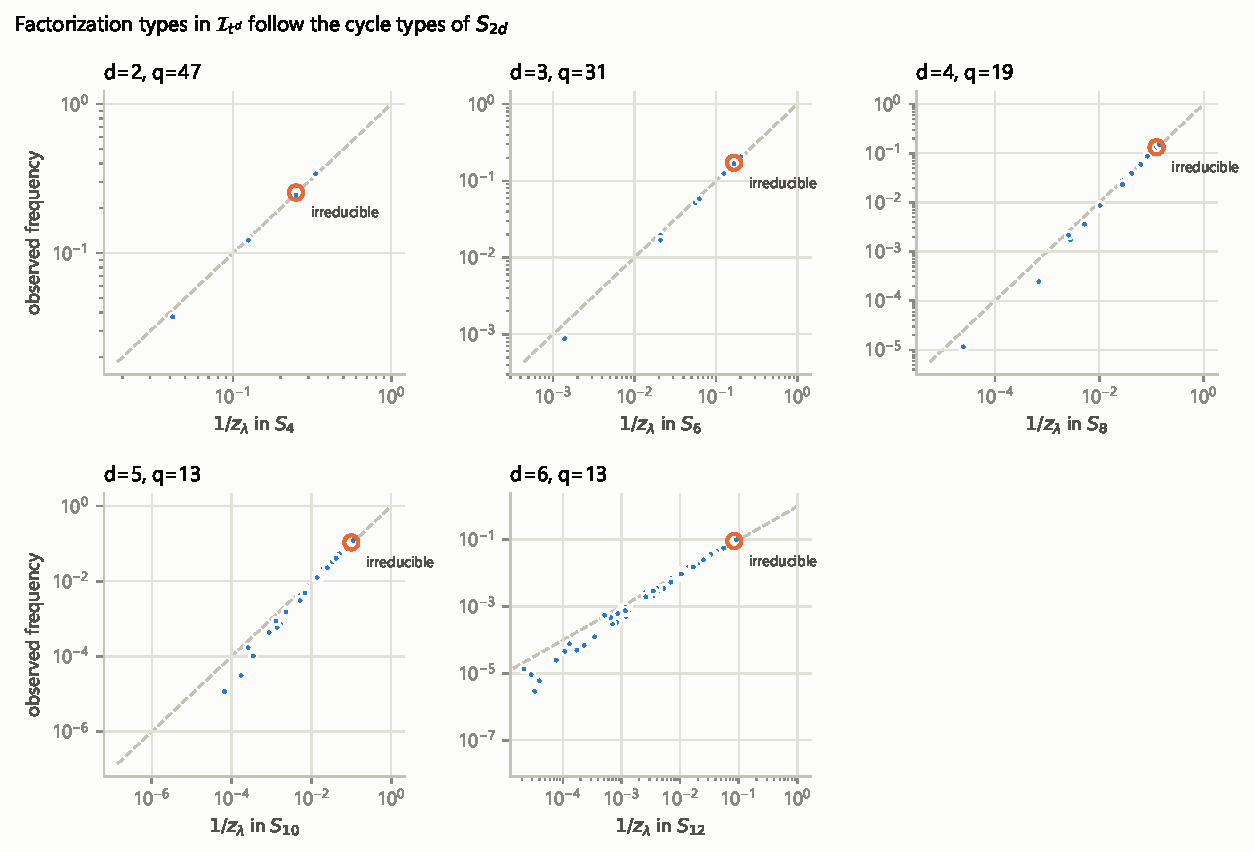
\includegraphics[width=\linewidth]{../figures/fig3_factorization_types.pdf}
\caption{Observed frequency of each factorization type in $\cI_{t^d}$ against the $S_{2d}$
cycle-type probability $1/z_\lambda$, as predicted by Theorem~\ref{thm:monodromy} and Chebotarev.
The ringed point is the irreducible type.}
\label{fig:cheb}
\end{figure}

% =====================================================================
\section{Discussion}\label{sec:discussion}
% =====================================================================

\paragraph{Where the difficulty lies.}
Theorem~1 shows that the analogue of Legendre's conjecture is a consequence of the Riemann
hypothesis for Hayes $L$-functions as long as $q\ge d-1$. Below that, the $d-2$ inverse roots of
each of the $q^{d-1}-1$ $L$-functions could in principle conspire, and nothing rules this out.
Over the integers the corresponding statement is that the Riemann hypothesis gives primes in
$[x,x+c\sqrt x\log x]$ but not in $[x,x+2\sqrt x]$. In both settings the missing input is
cancellation among zeros, not the location of zeros.

\paragraph{What the data suggest.}
The variance across intervals matches the random-matrix prediction of Keating and Rudnick even for
$q=3$, so the zeros of the relevant $L$-functions do behave independently in the range we can
compute. If that persists, empty intervals never occur (Section~\ref{sec:conjecture}).

\paragraph{Open problems.}
\begin{enumerate}[label=(\arabic*),nosep]
\item Prove Conjecture~\ref{conj:main} for one fixed $q$, for instance $q=2$, where the Legendre
      intervals form a thin and structured family.
\item Prove the Keating--Rudnick variance for fixed $q$ and $d\to\infty$, even in the Legendre range.
\item Extend Theorem~2 to $d=\AllQdNext$. This requires $q=5$ and $q=7$ with $d=\AllQdNext$ in full,
      about $2\times10^{11}$ and $4\times10^{13}$ irreducibility tests with the present method.
\item Higher powers: the intervals $\{f^k+s:\ \deg s\le(k-1)d\}$ for $k\ge3$, where the
      classical estimate covers a different range.
\end{enumerate}

\appendix
% =====================================================================
\section{Errata to version v5}\label{app:errata}
% =====================================================================
\begin{enumerate}[label=E\arabic*.,leftmargin=*]
\item \textbf{Novelty.} The main theorem of v5, $\Nirr=q^{d+1}/(2d)+O_d(q^{d+1/2})$, follows from the
      classical estimate of Theorem~1 and from \cite[Thm.~2.3]{BBR2015}, without the squarefree
      hypothesis and in every odd characteristic.
\item \textbf{Primitivity.} v5 applied ``imprimitive $\Leftrightarrow$ $F=g\circ h$'' to the Galois
      group of $F$ over $\Fqbar(\ba)$, where it does not hold as stated, and treated algebraic
      coefficients as free parameters. Fixed in Proposition~\ref{prop:primitive}.
\item \textbf{Transposition.} v5 misidentified the discriminant branches near $\ba=0$ and invoked
      Picard--Lefschetz without justification. Fixed in Proposition~\ref{prop:transposition}.
\item \textbf{Effective Chebotarev.} v5 stated the bound with the permutation sheaf, which detects
      linear factors, not $2d$-cycles, and cited an inapplicable theorem of \cite{Katz1988}.
\item \textbf{Betti-number bound.} v5 attributed to \cite[Thm.~12]{Katz2001} a bound for push-forwards
      of finite covers that is not there. The threshold $(8d)^{2d+6}$ was unproved.
\item \textbf{Other.} An error-term mix-up in the final step, a $j_!$/$j_*$ slip in the
      Grothendieck--Ogg--Shafarevich formula, wrong data for the Bary-Soroker citation, uncited
      references, version-history remarks in the body, and conclusions drawn from three small examples.
\end{enumerate}

% =====================================================================
\section{Corrections to version v6}\label{app:errata6}
% =====================================================================
\begin{enumerate}[label=F\arabic*.,leftmargin=*]
\item \textbf{Classical estimate omitted.} v6 did not mention the Hayes--Weil estimate
      (Theorem~1, \cite{Cohen2005,Hsu1996,Gao2021}). It gives $\Nirr\ge1$ for $q\ge d-1$ and error
      $O(dq^d)$. v6's Theorem~C ($q>1.65\times10^4$ for $d=4$), its Katz--Deligne bound and its
      bound via \cite{Sawin2021} (threshold about $(2d+2)^6$) are all superseded for existence;
      Table~\ref{tab:thresholds} compares them.
\item \textbf{Level 1/2.} v6 said that at level $1/2$ the Riemann hypothesis gives an error larger
      than the main term ``by a factor of order $d$''. The factor is $d/q$, as Theorem~1 shows.
\item \textbf{Novelty of the twisted identity.} The root variety is Sawin's $X_{n,m,\mathbf c}$, so
      Theorem~\ref{thm:identity} is a twisted form of his point count (this was added late in v6).
\item \textbf{Scope.} v6 described $q$ fixed, $d\to\infty$ as open without locating the open range;
      it is $q\le d-2$.
\end{enumerate}

\begin{table}[ht]
\centering\small
\begin{tabular}{rrrrr}
\toprule
$d$ & v5 claim (unproved) & Prop.~5.4 (Katz) & Cor.~5.3 (Cafure--Matera) & Prop.~5.5 (Sawin) \\
\midrule
1 & 7.2 & 2.2$^{\ast}$ & 0.8$^{\ast}$ & -- \\
2 & 12.0 & 5.7$^{\ast}$ & 0.9$^{\ast}$ & 4.7$^{\ast}$ \\
3 & 16.6 & 10.6$^{\ast}$ & 2.0$^{\ast}$ & 5.3$^{\ast}$ \\
4 & 21.1 & 16.3 & \textbf{4.2} & 5.9 \\
5 & 25.6 & 22.7 & 6.9 & \textbf{6.4} \\
6 & 30.3 & 29.7 & 9.9 & \textbf{6.8} \\
8 & 39.7 & 44.8 & 16.8 & \textbf{7.4} \\
10 & 49.5 & 61.4 & 24.8 & \textbf{7.9} \\
15 & 74.9 & 106.9 & 48.1 & \textbf{8.9} \\
20 & 101.4 & 157.0 & 74.7 & \textbf{9.7} \\
30 & 157.1 & 266.4 & 134.8 & \textbf{10.7} \\
40 & 215.4 & 384.8 & 201.4 & \textbf{11.4} \\
50 & 275.8 & 509.8 & 272.8 & \textbf{12.0} \\
\bottomrule
\multicolumn{5}{l}{\footnotesize $^{\ast}$\,not needed: Theorem~D gives $N_{\rm irr}\ge1$ for all admissible $q$.}
\end{tabular}
\caption{Thresholds $\log_{10}q_0(d)$ beyond which $\Nirr\ge1$ is proved. ``Classical'' is
Theorem~1 ($q_0=d-2$). The other rigorous columns are the bounds of v6: Katz's Betti bound with
Deligne, Cafure--Matera, and Sawin's theorem. ``v5'' was never proved.}
\label{tab:thresholds}
\end{table}

\begin{thebibliography}{99}

\bibitem{BHP2001}
R.\,C.~Baker, G.~Harman, J.~Pintz,
The difference between consecutive primes, II,
\textit{Proc.\ London Math.\ Soc.}\ \textbf{83} (2001), 532--562.

\bibitem{BBR2015}
E.~Bank, L.~Bary-Soroker, L.~Rosenzweig,
Prime polynomials in short intervals and in arithmetic progressions,
\textit{Duke Math.\ J.}\ \textbf{164} (2015), 277--295. arXiv:1302.0625.

\bibitem{CM2006}
A.~Cafure, G.~Matera,
Improved explicit estimates on the number of solutions of equations over a finite field,
\textit{Finite Fields Appl.}\ \textbf{12} (2006), 155--185.

\bibitem{Cohen2005}
S.\,D.~Cohen,
Explicit theorems on generator polynomials,
\textit{Finite Fields Appl.}\ \textbf{11} (2005), 337--357.

\bibitem{DM1996}
J.\,D.~Dixon, B.~Mortimer,
\textit{Permutation Groups}, GTM 163, Springer, 1996.

\bibitem{Fulton1998}
W.~Fulton, \textit{Intersection Theory}, 2nd ed., Springer, 1998.

\bibitem{Gao2021}
Z.~Gao,
Improved error bounds for the number of irreducible polynomials and self-reciprocal irreducible
monic polynomials with prescribed coefficients over a finite field, arXiv:2109.14154, 2021.

\bibitem{Ha2016}
J.~Ha,
Irreducible polynomials with several prescribed coefficients,
\textit{Finite Fields Appl.}\ \textbf{40} (2016), 10--25.

\bibitem{Hayes1965}
D.\,R.~Hayes,
The distribution of irreducibles in $GF[q,x]$,
\textit{Trans.\ Amer.\ Math.\ Soc.}\ \textbf{117} (1965), 101--127.

\bibitem{Hsu1996}
C.\,N.~Hsu,
The distribution of irreducible polynomials in $\mathbb F_q[t]$,
\textit{J.\ Number Theory} \textbf{61} (1996), 85--96.

\bibitem{Katz1988}
N.\,M.~Katz,
\textit{Gauss Sums, Kloosterman Sums, and Monodromy Groups},
Ann.\ of Math.\ Stud.\ 116, Princeton Univ.\ Press, 1988.

\bibitem{Katz2001}
N.\,M.~Katz,
Sums of Betti numbers in arbitrary characteristic,
\textit{Finite Fields Appl.}\ \textbf{7} (2001), 29--44.

\bibitem{KR2014}
J.\,P.~Keating, Z.~Rudnick,
The variance of the number of prime polynomials in short intervals and in residue classes,
\textit{Int.\ Math.\ Res.\ Not.}\ 2014, 259--288. arXiv:1204.0708.

\bibitem{LL2016}
M.~Lal\'in, O.~Larocque,
The number of irreducible polynomials with the first two prescribed coefficients over a finite field,
\textit{Rocky Mountain J.\ Math.}\ \textbf{46} (2016), 1587--1618.

\bibitem{LN1997}
R.~Lidl, H.~Niederreiter,
\textit{Finite Fields}, 2nd ed., Cambridge Univ.\ Press, 1997.

\bibitem{MY2016}
G.~McGuire, E.\,S.~Y\i lmaz,
The number of irreducible polynomials with the first two coefficients fixed over finite fields of
odd characteristic, arXiv:1609.02314.

\bibitem{Muller1995}
P.~M\"uller,
Primitive monodromy groups of polynomials, in
\textit{Recent Developments in the Inverse Galois Problem}, Contemp.\ Math.\ \textbf{186},
Amer.\ Math.\ Soc., 1995, 385--401.

\bibitem{Pollack2013}
P.~Pollack,
Irreducible polynomials with several prescribed coefficients,
\textit{Finite Fields Appl.}\ \textbf{22} (2013), 70--78.

\bibitem{Sawin2021}
W.~Sawin,
Square-root cancellation for sums of factorization functions over short intervals in function fields,
\textit{Duke Math.\ J.}\ \textbf{170} (2021), 997--1026. arXiv:1809.05137.

\bibitem{SawinShusterman2022}
W.~Sawin, M.~Shusterman,
On the Chowla and twin primes conjectures over $\mathbb F_q[T]$,
\textit{Ann.\ of Math.}\ \textbf{196} (2022), no.~2. arXiv:1808.04001.

\bibitem{Turnwald1995}
G.~Turnwald,
On Schur's conjecture,
\textit{J.\ Austral.\ Math.\ Soc.\ Ser.~A} \textbf{58} (1995), 312--357.

\end{thebibliography}
\end{document}
